\documentclass[11pt,a4paper]{article}

% ---------- Packages ----------
\usepackage[utf8]{inputenc}
\usepackage[T1]{fontenc}
\usepackage[margin=2.4cm]{geometry}
\usepackage{amsmath,amssymb,amsthm}
\usepackage{graphicx}
\usepackage{booktabs}
\usepackage{multirow}
\usepackage{array}
\usepackage{caption}
\usepackage{subcaption}
\usepackage{xcolor}
\usepackage{hyperref}
\usepackage[protrusion=true,expansion=false]{microtype}
\usepackage{enumitem}
\usepackage{listings}
\usepackage{titlesec}
\usepackage{fancyhdr}

% ---------- Hyperref ----------
\hypersetup{
  colorlinks=true,
  linkcolor=black!70!blue,
  urlcolor=blue!60!black,
  citecolor=black!70!blue,
}

% ---------- Headings ----------
\titleformat{\section}{\large\bfseries}{\thesection.}{0.6em}{}
\titleformat{\subsection}{\normalsize\bfseries}{\thesubsection}{0.5em}{}
\titlespacing*{\section}{0pt}{1.0em}{0.4em}
\titlespacing*{\subsection}{0pt}{0.7em}{0.2em}

\setlength{\parindent}{0pt}
\setlength{\parskip}{0.4em}
\captionsetup{font=small,labelfont=bf,skip=4pt}

% ---------- Listings ----------
\definecolor{codegray}{rgb}{0.45,0.45,0.45}
\lstset{
  basicstyle=\ttfamily\footnotesize,
  commentstyle=\color{codegray},
  keywordstyle=\color{blue!70!black},
  showstringspaces=false,
  breaklines=true,
  frame=none,
}

% ---------- Title block ----------
\title{\vspace{-1.5em}\textbf{Mortgage Prepayment Risk Modeling:\\
From Kaplan--Meier to Deep Survival Analysis}\\[0.3em]
\large IR\&C Assignment 3 --- Spring 2026}
\author{Kassziopeia\\\small MTH 9877 --- Interest Rate and Credit Models, Baruch College}
\date{May 2026}

% ---------- Document ----------
\begin{document}
\maketitle
\vspace{-1.2em}

% =================================================================
\section{Introduction}
% =================================================================

This project develops a data-driven understanding of mortgage prepayment risk on the Freddie Mac Single-Family Loan-Level Dataset, applying classical survival analysis, machine learning, and deep survival models to a single 30-year fixed-rate mortgage population.

The full standard dataset contains 31{,}688{,}129 loans originated between 1999 and 2025, of which 68.6\% have prepaid by the performance cutoff date. We focus exclusively on the prepayment event; non-prepayment terminations (default, third-party sale, REO disposition) are treated as right-censored under a cause-specific framing. The study covers four parts:

\begin{itemize}[leftmargin=1.2em,itemsep=2pt,topsep=2pt]
\item \textbf{Part A:} Kaplan--Meier survival estimation on the full population, stratified by FICO, LTV, vintage, and loan purpose.
\item \textbf{Part B:} Classical Cox proportional hazards model with origination covariates, plus a vintage-macro extension that joins FRED macroeconomic series at origination.
\item \textbf{Part C:} Machine learning models (Logistic Regression, Random Forest, LightGBM) for horizon-specific binary prediction $P(\text{prepaid by } T \mid X)$, with a Cox baseline for comparison.
\item \textbf{Part D:} Deep Cox model (DeepSurv) replacing the linear predictor of the Cox model with a feed-forward neural network, plus a depth-0 linear-Cox-via-SGD ablation to isolate the gain from nonlinearity.
\end{itemize}

\textbf{Headline finding.} The Deep Cox model achieves AUC = 0.729 at the 60-month horizon versus 0.685 for the matched-architecture linear baseline ($\Delta\text{AUC} = +0.044$). The gap widens monotonically with horizon, from $+0.003$ at $T{=}12$ to $+0.045$ at $T{=}60$, indicating that nonlinear interactions between borrower covariates and time accumulate over the loan's life. Deep Cox is the best-performing model at every horizon $\geq 24$ months, beating tree-based methods and logistic regression.

\subsection{Background and prior work}

\textbf{Mortgage prepayment} is the early termination of a loan when a borrower refinances, sells the property, or pays off the balance. From a mortgage-backed-security investor's perspective, prepayment is a competing risk to default: the cash flow ends in either case, but the recovery economics differ. Modeling prepayment timing is therefore central to the valuation and hedging of MBS, to the design of credit risk transfer transactions, and to portfolio-level asset-liability management at the GSEs and large servicers.

\textbf{Classical models.} The empirical mortgage literature (Schwartz \& Torous 1989; Stanton 1995; Deng--Quigley--Van Order 2000) has long used Cox proportional hazards models with hand-engineered covariates: original interest rate, FICO, LTV, loan age, prepayment incentive (current rate minus mortgage rate). These models are tractable and interpretable but assume the hazard ratio is constant over the loan's life --- the proportional hazards assumption.

\textbf{Deep survival models.} Katzman et al.\ (2018, DeepSurv) and Kvamme et al.\ (2019, pycox) extended the Cox framework by replacing the linear predictor with a neural network. Sadhwani, Giesecke \& Sirignano (2021), in the canonical paper for this domain, applied a five-layer network to 120M+ CoreLogic mortgages with 272 covariates including zip-code-level macro and demographic data. They documented strong nonlinear effects across multiple competing outcomes, with prepayment showing the largest gains over linear baselines. Our project replicates the methodological core of that paper on the much smaller Freddie Mac dataset.

% =================================================================
\section{Data and Methodology}
% =================================================================

\subsection{Survival table construction}

The raw Freddie Mac data is delivered as quarterly origination files plus monthly performance files, totaling tens of GB. We construct a single \emph{survival table} of 31.7M loans by:
(i) aggregating each loan's monthly performance to a single record with \texttt{Duration} (months from first payment to terminal observation), \texttt{Event\_Prepay} (binary), and \texttt{Terminated} (binary);
(ii) deriving an explicit \texttt{CreditTerminated} indicator distinguishing credit-related exits (Zero Balance Code 03, 09) from voluntary prepayment (ZBC 01); and
(iii) cleaning Freddie Mac's sentinel codes (DTI = 999, MI = 999, etc.) to NaN.
Categorical covariates are top-K-encoded (e.g., top-15 servicers) with rare levels collapsed to ``Other''.

\subsection{Targets and split}

For Parts C and D we evaluate at horizons $T \in \{12, 24, 36, 60\}$ months. Targets are constructed under the cause-specific framing: a loan that prepays by $T$ is a positive (1); a loan observed through $T$ without prepayment or competing termination is a negative (0); a loan with competing termination at $\text{Duration} \leq T$ or right-censored before $T$ is excluded (NaN). This is the standard cause-specific framing for competing risks~\cite{kalbfleischprentice}.

The train/test split is by vintage: \textbf{train} = vintages $\leq 2014$ (full crisis and pre-crisis cycle), \textbf{test} = vintages 2015--2019 (out-of-sample post-crisis). For Part D, we additionally carve a 10\% validation slice from the training set \emph{before} feature transformation, used only for early stopping. The split is persisted as \texttt{canonical\_split.parquet} so that Parts C and D evaluate on identical test rows. A 10\% random sample (3.17M loans) is used for Parts B--D to fit memory; the test set is 597{,}205 loans after restricting to vintages 2015--2019.

\subsection{Feature engineering}

The 39 origination columns expand to a 68-feature matrix after encoding:

\begin{itemize}[leftmargin=1.2em,itemsep=2pt,topsep=2pt]
\item \textbf{Continuous covariates} (FICO, LTV, original interest rate, original UPB, DTI) are z-scored using means and standard deviations fit on the training set only. Missing values are imputed with the training-set median, with a paired binary ``missing'' flag added as an additional feature so the model can learn whether missingness itself is informative (it is for DTI, which equals 999 for Relief Refinance loans).
\item \textbf{Low-cardinality categoricals} (Loan Purpose, Occupancy, Channel, Property Type, First-Time Homebuyer) are one-hot encoded with one reference level dropped.
\item \textbf{High-cardinality categoricals} (Seller Name, Servicer Name, Property State) are top-15 encoded: the 15 most-common levels in the training set get their own indicator, with all rare levels collapsed to ``Other''.
\item \textbf{Macro covariates} (Part B only) are joined at \texttt{FirstPaymentDate} and z-scored.
\end{itemize}

All encoders (top-K level lists, medians, scaler stats) are fit on the training set only and persisted as \texttt{encoders.pkl} for Part D to reuse, ensuring identical preprocessing across parts. This was a critical fix discovered during cross-AI code review: the original Part C version was fitting encoders on the full sample before splitting, which leaked test-set distribution into training-set medians.

\subsection{One key equation}

Throughout Parts B and D, the survival function $S(t \mid X)$ is parameterized by Cox proportional hazards:
\begin{equation}
\lambda(t \mid X) \;=\; \lambda_0(t) \cdot \exp\!\bigl(f_\theta(X)\bigr),
\label{eq:cox}
\end{equation}
where $\lambda_0(t)$ is a non-parametric baseline hazard (estimated by Breslow's estimator) and $f_\theta$ is either a linear predictor $X^\top \beta$ (classical Cox) or a feed-forward neural network (Deep Cox). The model is fit by maximum partial likelihood; the likelihood does not depend on $\lambda_0$, which is recovered post-hoc.

% =================================================================
\section{Part A --- Kaplan--Meier Survival Estimation}
% =================================================================

\textbf{Setup.} We fit the non-parametric Kaplan--Meier estimator on the full 31.7M-loan population (no sampling). For prepayment KM, all non-prepay outcomes are pooled as right-censored: 9{,}141{,}814 still-active loans plus 797{,}541 credit-related and other terminations, for 9{,}939{,}355 censored observations (31.4\%) versus 21{,}748{,}774 prepayment events (68.6\%).

\textbf{Overall survival.} The median time to prepayment is 50 months. The survival curve is steep in the first three years and decays through:
$S(12){=}0.898,\; S(36){=}0.623,\; S(60){=}0.427,\; S(120){=}0.155,\; S(240){=}0.037$.

\textbf{Hazard rates.} The discrete monthly hazard $h(t) = 1 - S(t{+}1)/S(t)$ ramps from $\approx 0.97\%$ at $t{=}6$ to $\approx 1.4\%$ at $t{=}12$, then plateaus around $1.5\%$ to $1.7\%$ monthly (annualized $\approx 17\%{-}18\%$) from year 2 onwards. The annualized rate of $\sim 18\%$ matches industry SMM benchmarks.

\begin{figure}[h]
\centering
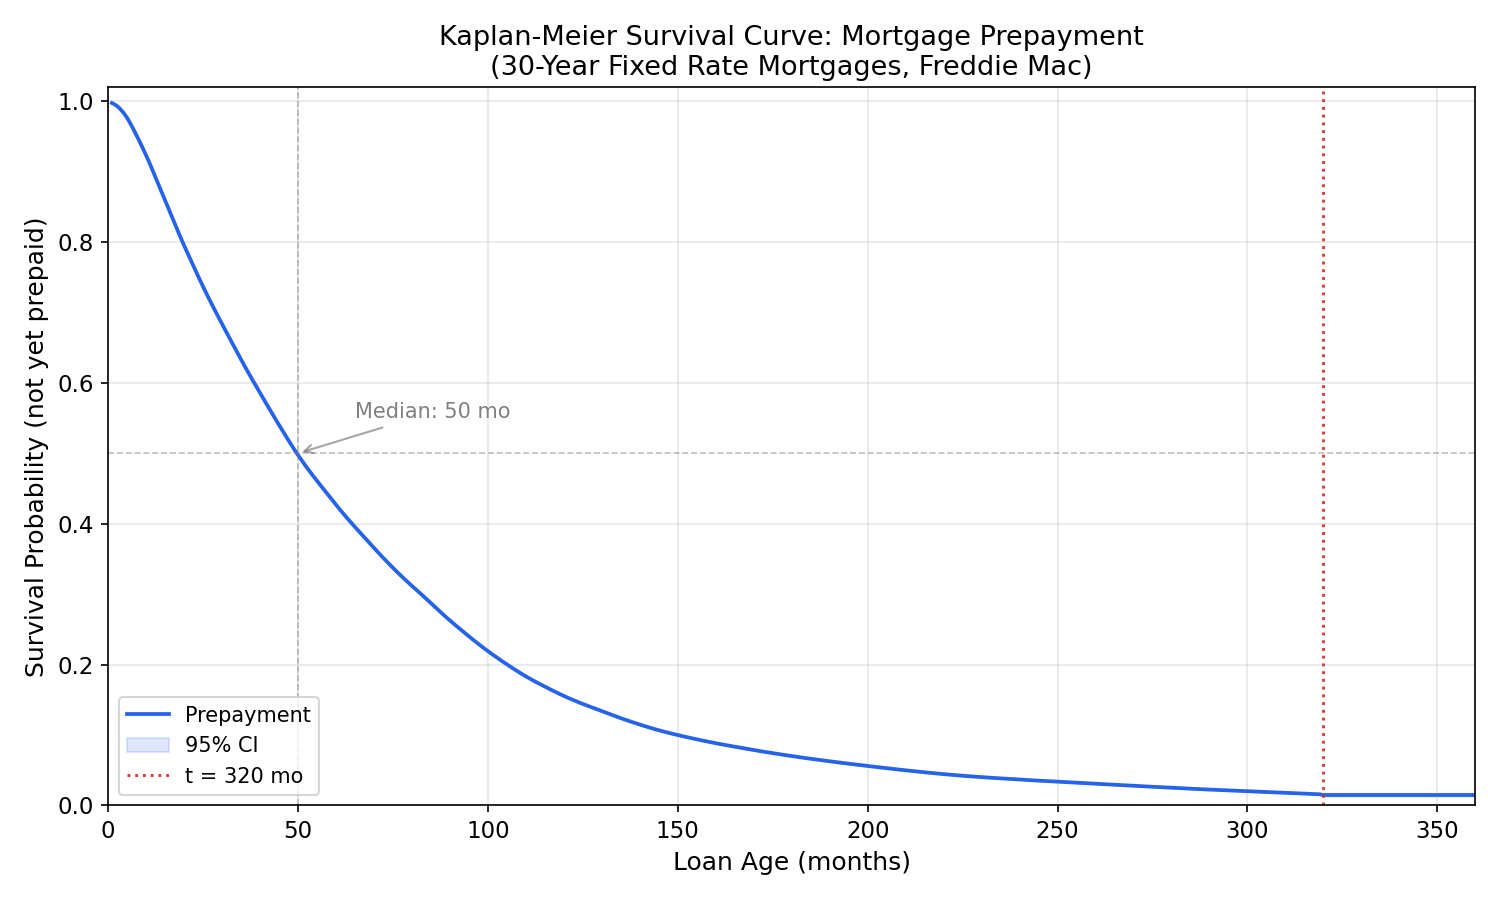
\includegraphics[width=0.49\textwidth]{plots/A_km_overall.png}\hfill
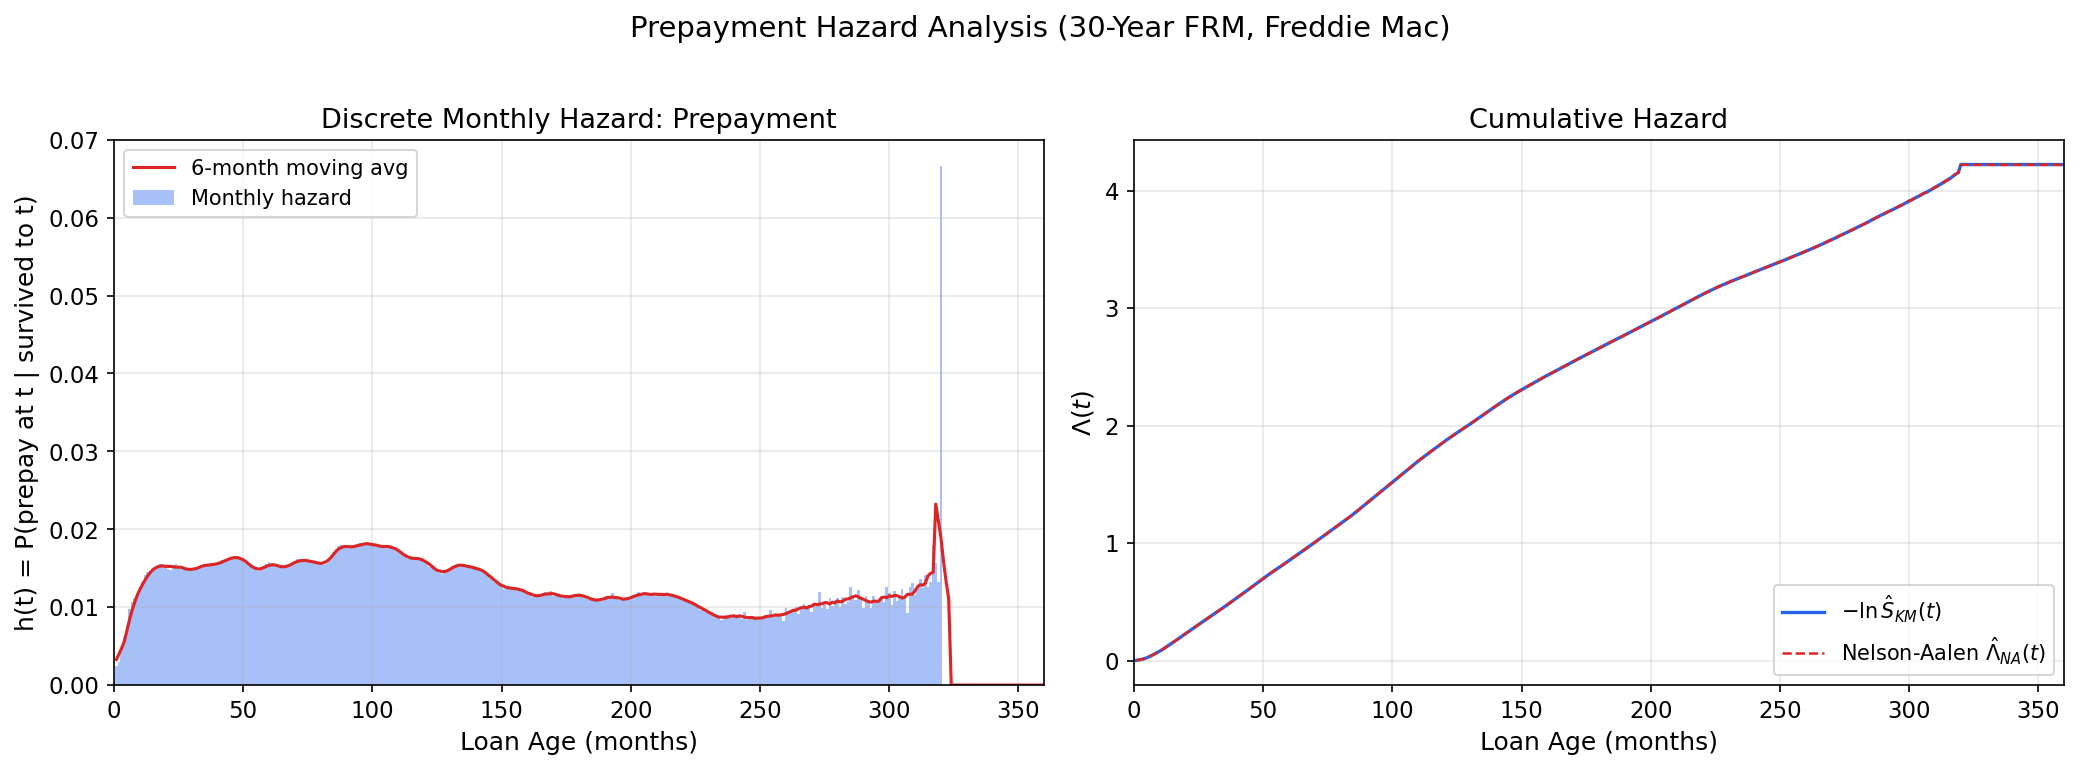
\includegraphics[width=0.49\textwidth]{plots/A_hazard_overall.png}
\caption{\textbf{Part A.} Left: KM survival curve on the full population (31.7M loans). Right: implied discrete monthly hazard from KM and the Nelson--Aalen cumulative hazard estimator. The two cumulative-hazard estimates ($-\log S_{\text{KM}}$ and $\hat H_{\text{NA}}$) agree closely as expected.}
\end{figure}

\textbf{Stratified curves.} The strongest single-variable effect is by \emph{vintage}: 1999--2003 loans prepay almost completely (96.3\%) with median 29 months, while 2020+ loans show only 16\% prepayment with median undefined (right-censored before reaching 50\%). LTV and FICO show modest, monotone gradients. Loan purpose is more nuanced --- no-cash-out refis prepay slightly more (70\%) than purchase loans (67\%) or cash-out refis (70\%), but with shifted timing.

\begin{figure}[h]
\centering
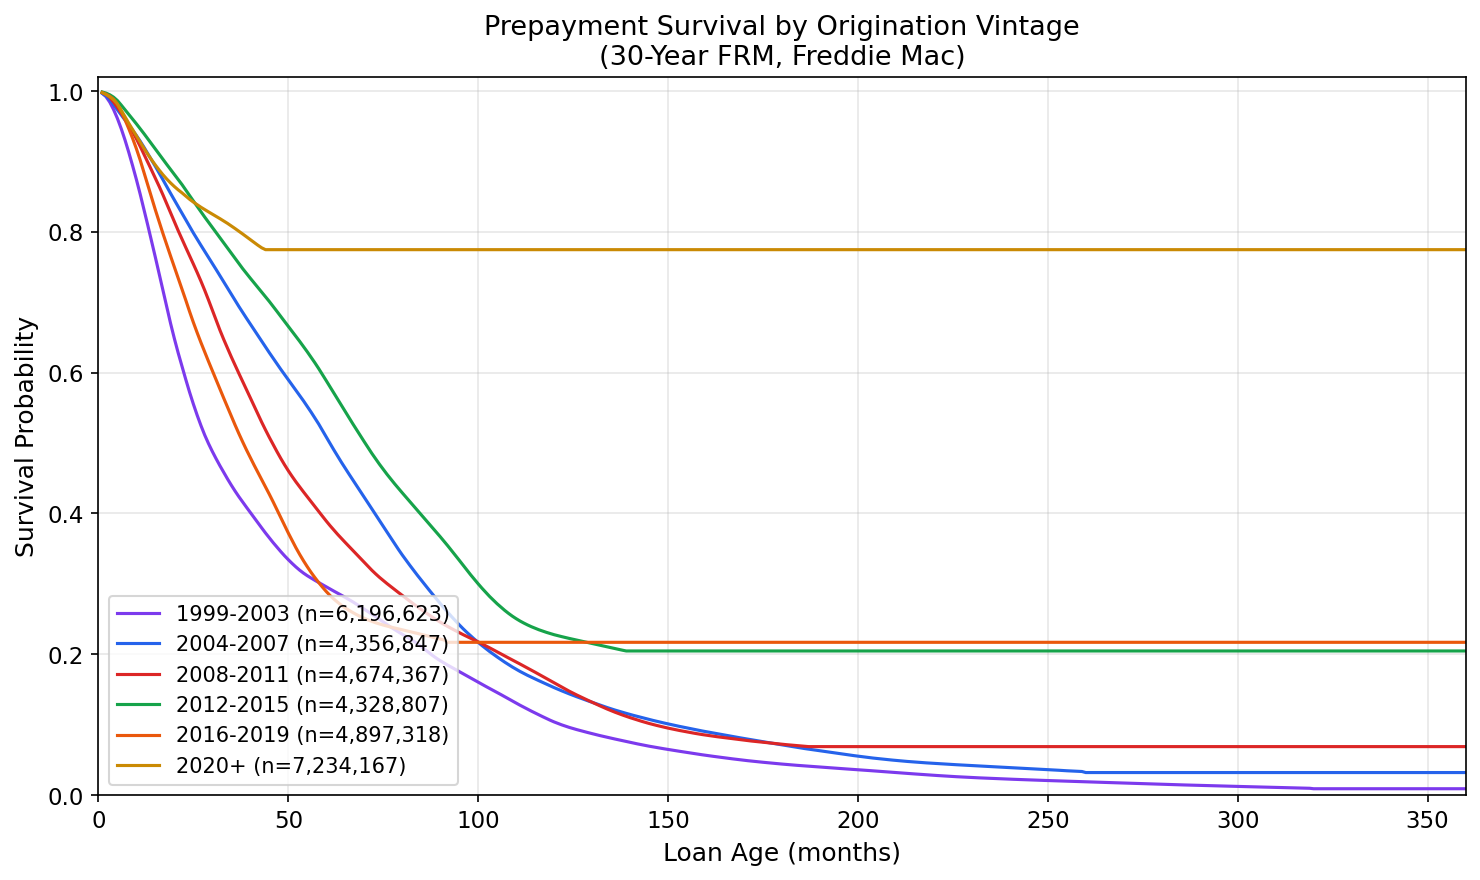
\includegraphics[width=0.49\textwidth]{plots/A_km_by_vintage.png}\hfill
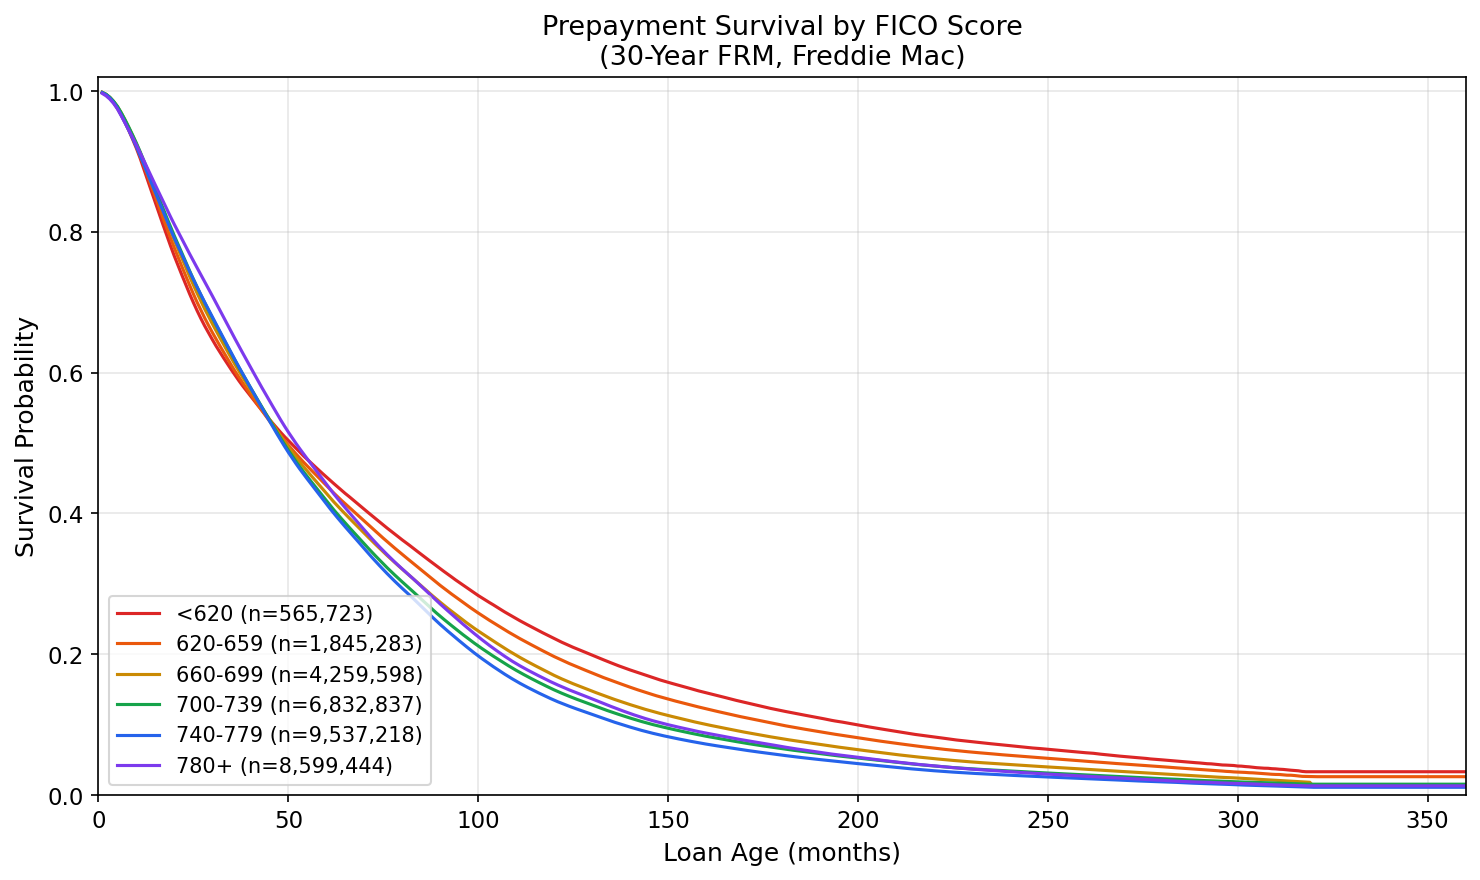
\includegraphics[width=0.49\textwidth]{plots/A_km_by_fico.png}
\caption{\textbf{Part A stratification.} Left: by vintage cohort (rate environment dominates). Right: by FICO bucket (more modest, monotone gradient).}
\end{figure}

% =================================================================
\section{Part B --- Cox Proportional Hazards}
% =================================================================

\textbf{Setup.} 5\% sample (1.58M loans, 1.08M events). 15 origination covariates (continuous standardized to z-scores; categorical as one-hot dummies with one reference). Fit via lifelines with $\ell_2$ penalizer 0.001.

\textbf{Base model.} Concordance index 0.6257 (modest; Cox is a one-parameter-per-covariate model on highly nonlinear data). The largest hazard ratios:
\begin{itemize}[leftmargin=1.2em,itemsep=2pt,topsep=2pt]
\item \textbf{Original interest rate} (z): $\text{HR} = 1.58$ --- the dominant prepayment driver. Borrowers with high origination rates have the most refinancing incentive when rates fall.
\item \textbf{Original UPB} (z): $\text{HR} = 1.29$ --- larger loans prepay more, consistent with refinancing fixed costs being amortized over larger principal.
\item \textbf{Investment property}: $\text{HR} = 0.80$ --- investors prepay less (lower mobility, different tax treatment).
\item \textbf{DTI missing}: $\text{HR} = 0.82$ --- DTI=999 is the Relief Refinance flag (FAQ Q67); these loans behave differently.
\end{itemize}

\textbf{Vintage-macro extension.} Adding four FRED macroeconomic series joined at origination (\texttt{FirstPaymentDate}) raises concordance to 0.6428 (improvement $\Delta C = +0.017$, $\Delta\text{AIC} = -28{,}510$):
\begin{itemize}[leftmargin=1.2em,itemsep=2pt,topsep=2pt]
\item \textbf{10y Treasury rate at origination}: $\text{HR} = 0.78$ --- borrowers whose loans were originated when long rates were high subsequently prepay more (relative to those originated in low-rate environments), because they are more likely to encounter a rate-cut refinance opportunity.
\item \textbf{HPI YoY at origination}: $\text{HR} = 0.89$ --- loans originated during housing booms prepay less than those originated in flat/declining markets.
\item \textbf{Unemployment at origination}: $\text{HR} = 0.89$ --- consistent with the Sadhwani et al.\ 2021 ``labor market shock'' channel.
\end{itemize}

\textbf{Caveat.} These are vintage-macro covariates --- the macro state at the time of origination, \emph{not} time-varying through the loan's life. A truly dynamic Cox model with time-dependent covariates would require the full loan-month panel, which exceeds our memory budget.

\textbf{Proportional hazards diagnostic.} The Schoenfeld residual test rejects PH for 12 of 15 covariates at $\alpha = 0.05$. This is the standard finding on mortgage data and is the principal motivation for moving beyond Cox.

\begin{figure}[h]
\centering
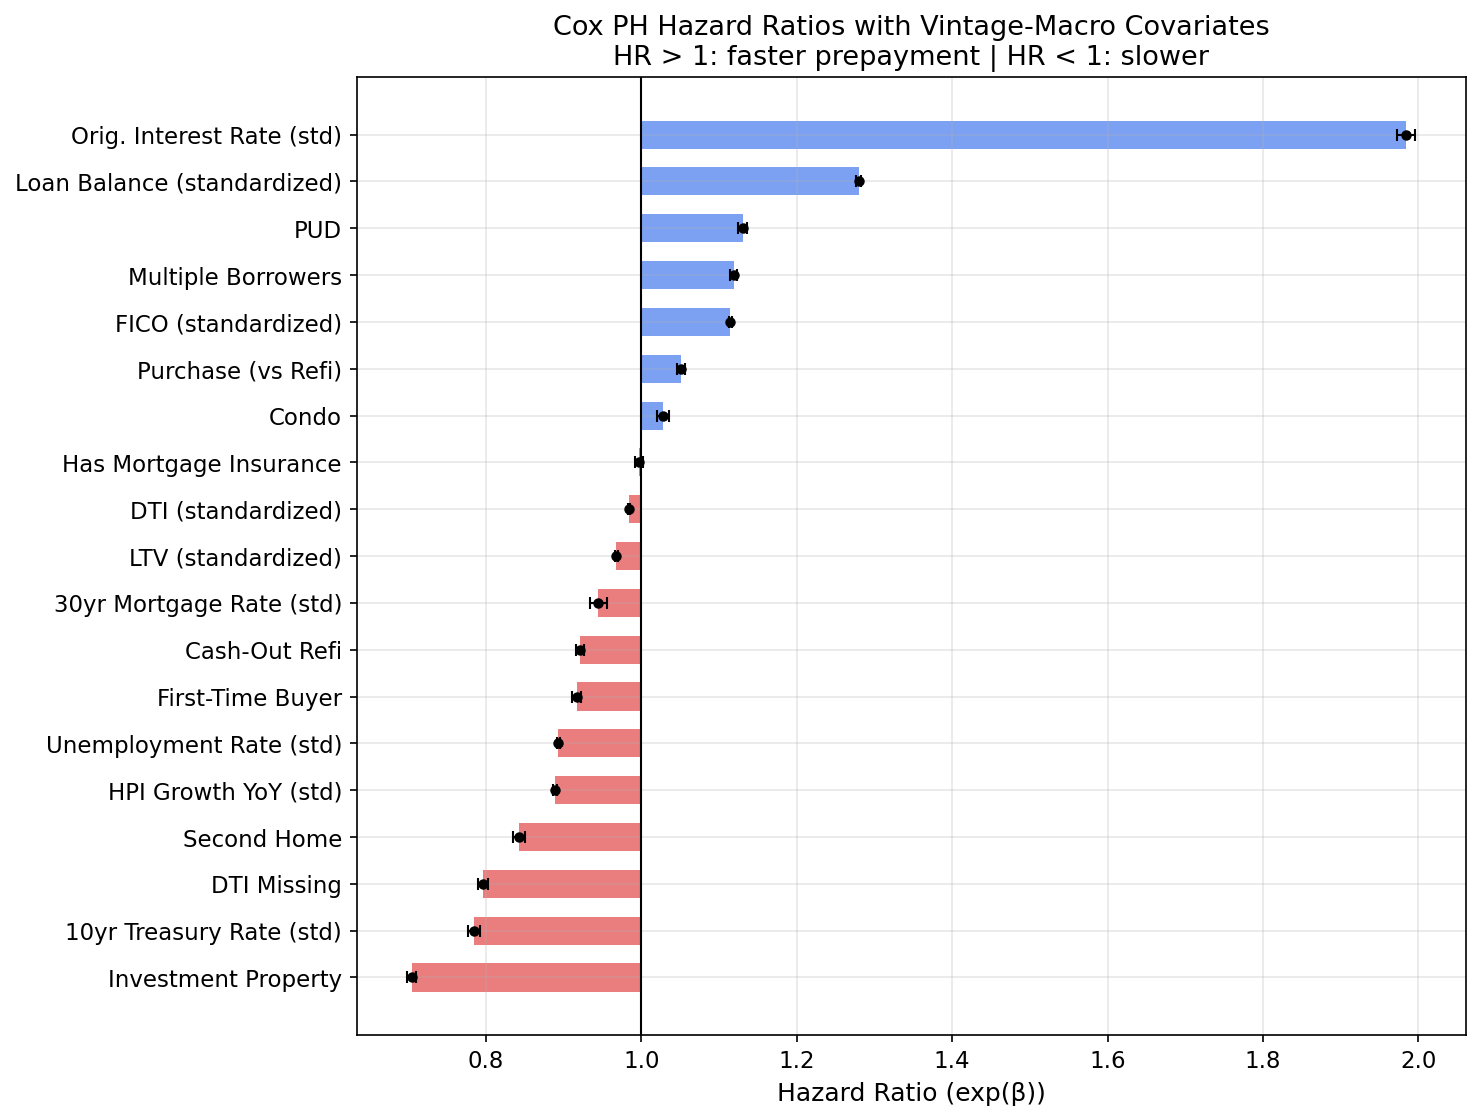
\includegraphics[width=0.49\textwidth]{plots/B_hazard_ratios_macro.png}\hfill
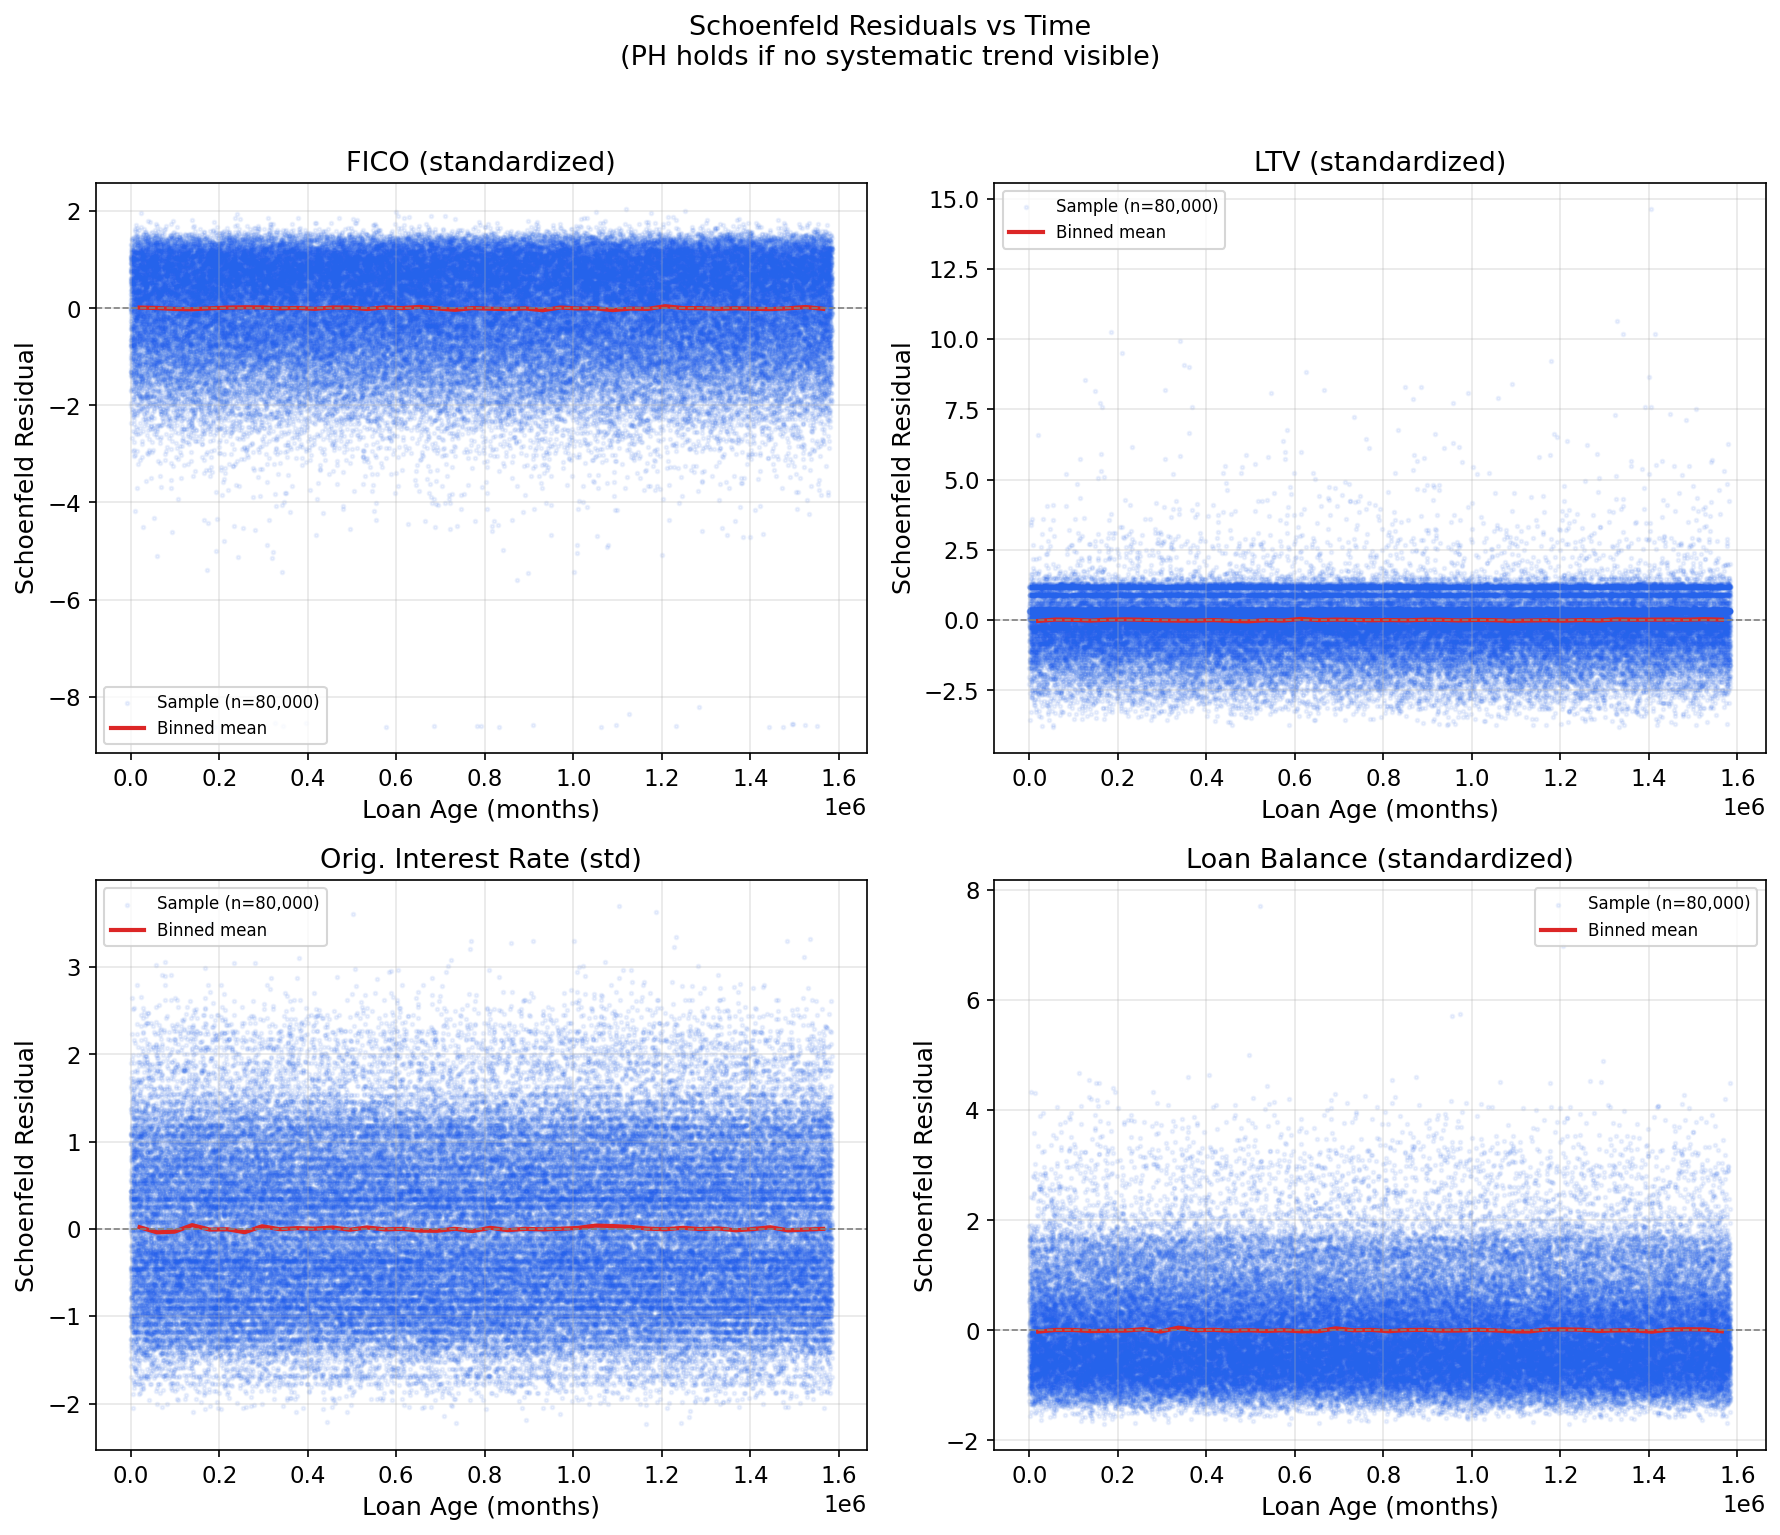
\includegraphics[width=0.49\textwidth]{plots/B_ph_test.png}
\caption{\textbf{Part B.} Left: hazard ratios from the macro Cox model (HR$>$1 increases prepayment hazard). Right: Schoenfeld PH-test p-values --- 12/15 covariates show evidence of PH violation.}
\end{figure}

% =================================================================
\section{Part C --- Machine Learning Models}
% =================================================================

\textbf{Setup.} 10\% sample, 1.85M training and 597k test loans, 68 features post one-hot. We fit four models: Logistic Regression with $\ell_2$ regularization (using its own scaler internally), Random Forest (200 trees), LightGBM (early-stopping via held-out validation), and a Cox baseline using lifelines. Each model is fit per-horizon as a binary classifier targeting $\mathbf{1}\{\text{prepaid by } T\}$, with cause-specific exclusions as described.

\textbf{Out-of-sample AUC.}

\begin{center}
\small
\begin{tabular}{lcccc}
\toprule
Model & T=12 & T=24 & T=36 & T=60 \\
\midrule
Cox        & 0.6635 & 0.6571 & 0.6596 & 0.6650 \\
Random Forest & 0.6706 & 0.6519 & 0.6718 & 0.6803 \\
LightGBM   & 0.6805 & 0.6738 & 0.6899 & 0.6825 \\
LogReg     & 0.6908 & 0.6670 & 0.6837 & 0.7043 \\
\bottomrule
\end{tabular}
\end{center}

The four models cluster in the 0.65--0.70 AUC band. Logistic regression is competitive --- in fact best at $T{=}12$ and $T{=}60$ --- which suggests that the marginal effects in the data are largely linear-additive in z-scored covariates and that tree models' axis-aligned splits don't unlock much extra signal at these horizons. LightGBM has the best Brier scores and is consistently top-2.

\textbf{Calibration.} All four models are reasonably well-calibrated, with LightGBM and LogReg showing the tightest fit to the diagonal. Cox is slightly under-confident at the high end (the linear-predictor model can't push probabilities very close to 1 even when warranted).

\textbf{Top-decile lift.} For an investor interested in identifying loans most likely to prepay, the lift in the top decile is most informative at moderate horizons: at $T{=}12$, the top decile contains 27.6\% prepayments (LightGBM) versus a 10.75\% base rate, for a lift of 2.57$\times$. Logistic regression achieves nearly identical lift (2.54$\times$). The lift saturates at long horizons because the base prepayment rate exceeds 70\% at $T{=}60$ --- there is simply not much room in the top decile for additional concentration.

\begin{figure}[h]
\centering
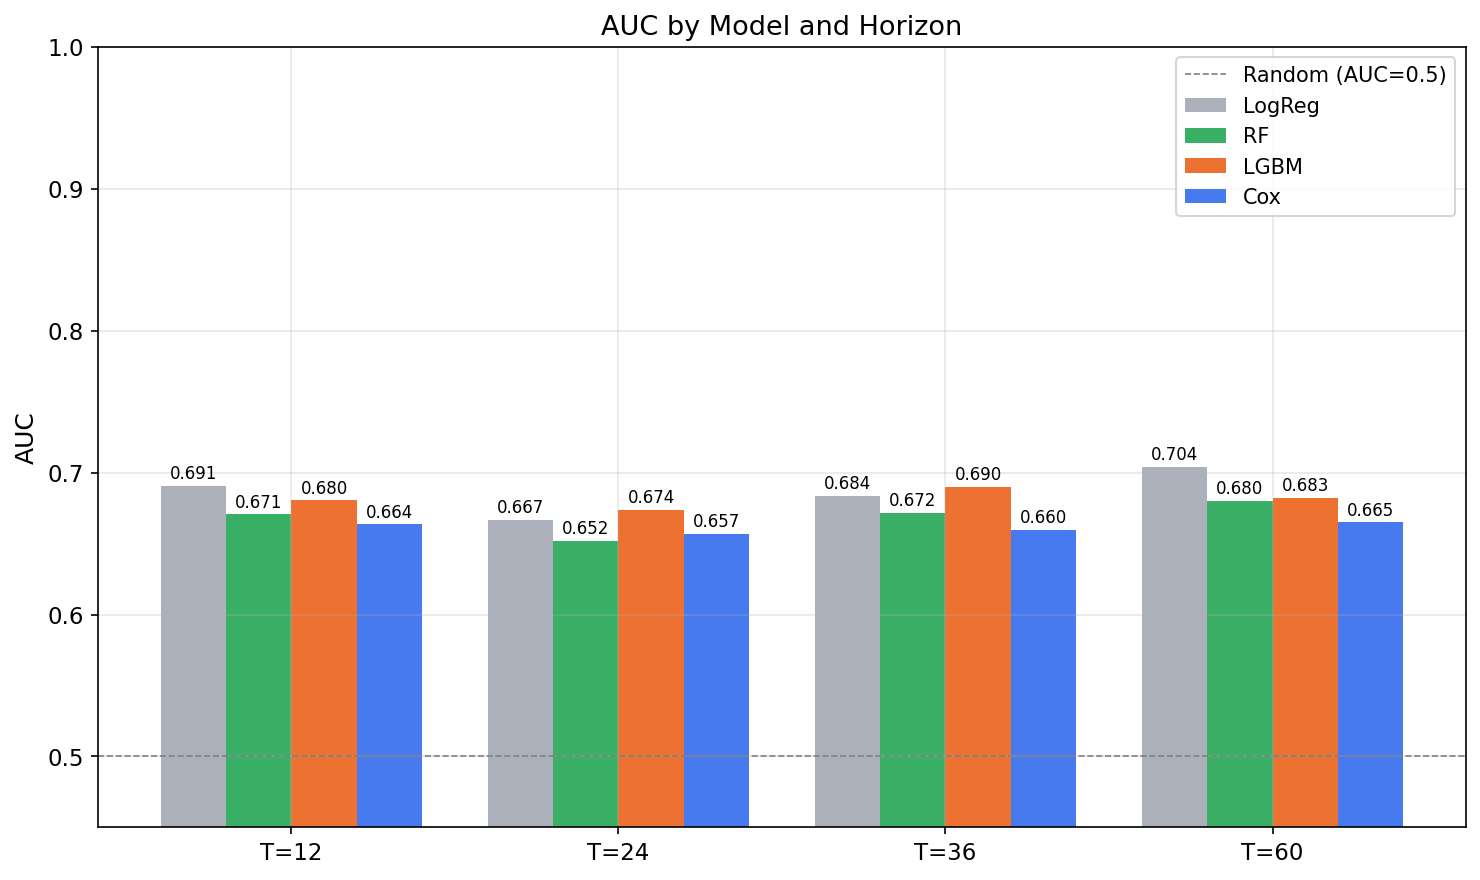
\includegraphics[width=0.49\textwidth]{plots/C_auc_by_horizon.png}\hfill
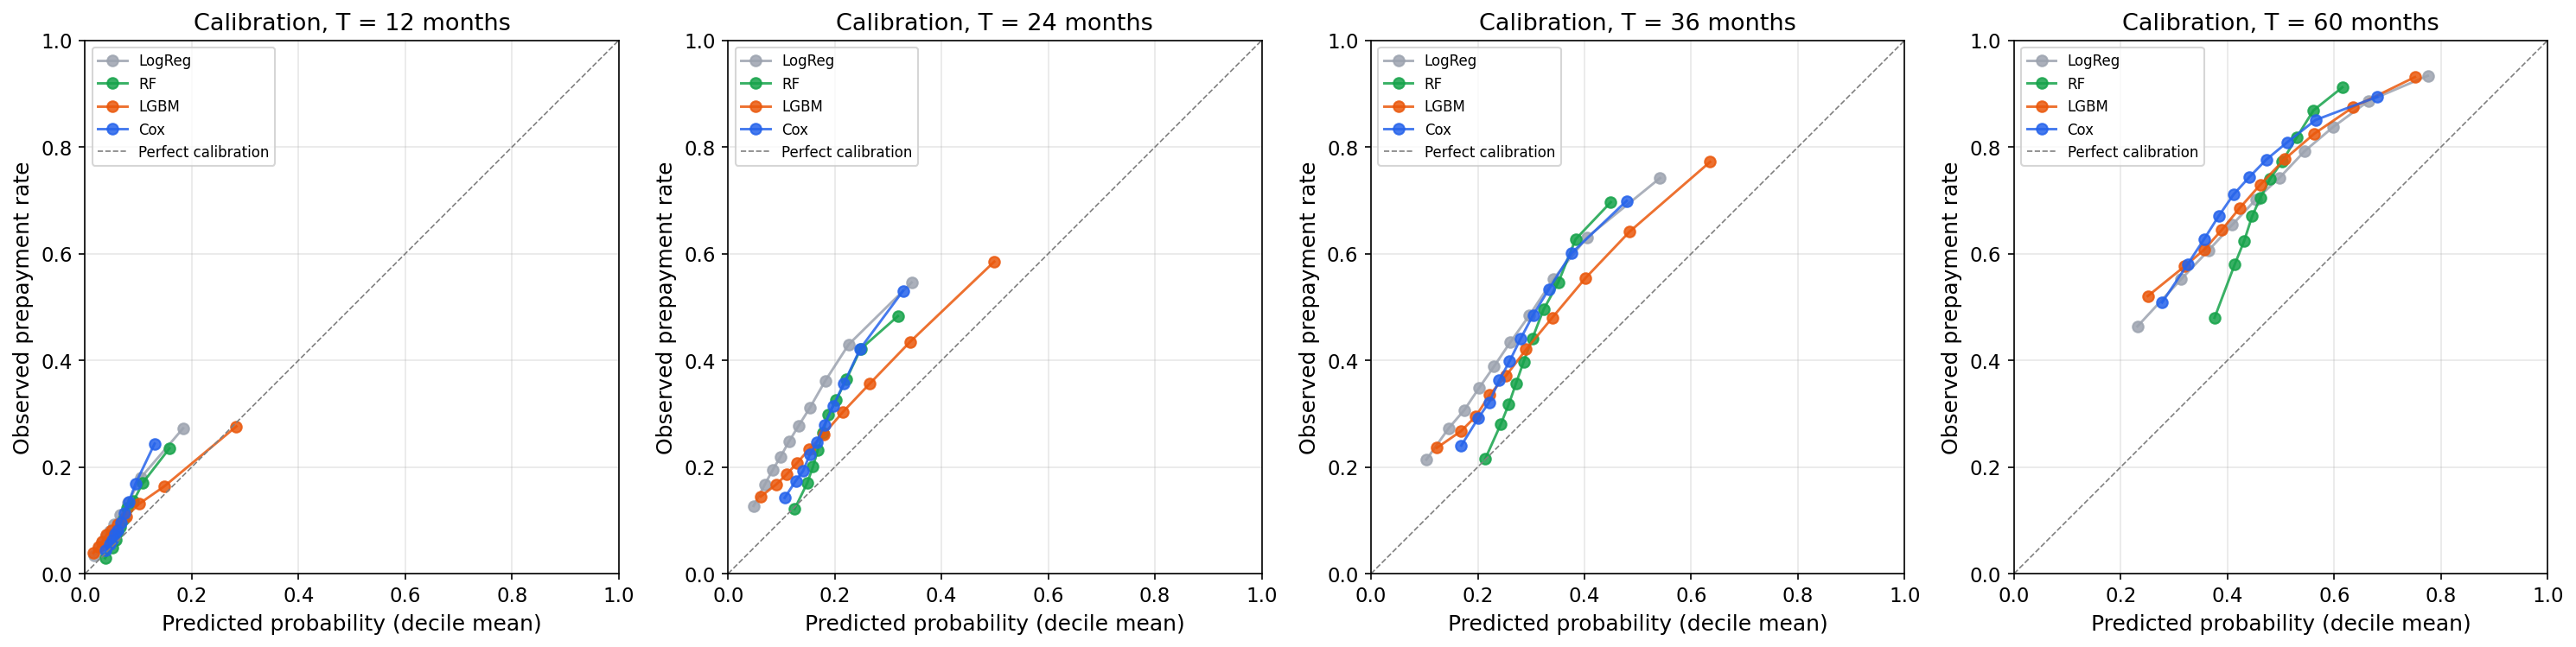
\includegraphics[width=0.49\textwidth]{plots/C_calibration.png}
\caption{\textbf{Part C.} Left: AUC by model and horizon. Right: decile calibration plot.}
\end{figure}

\begin{figure}[h]
\centering
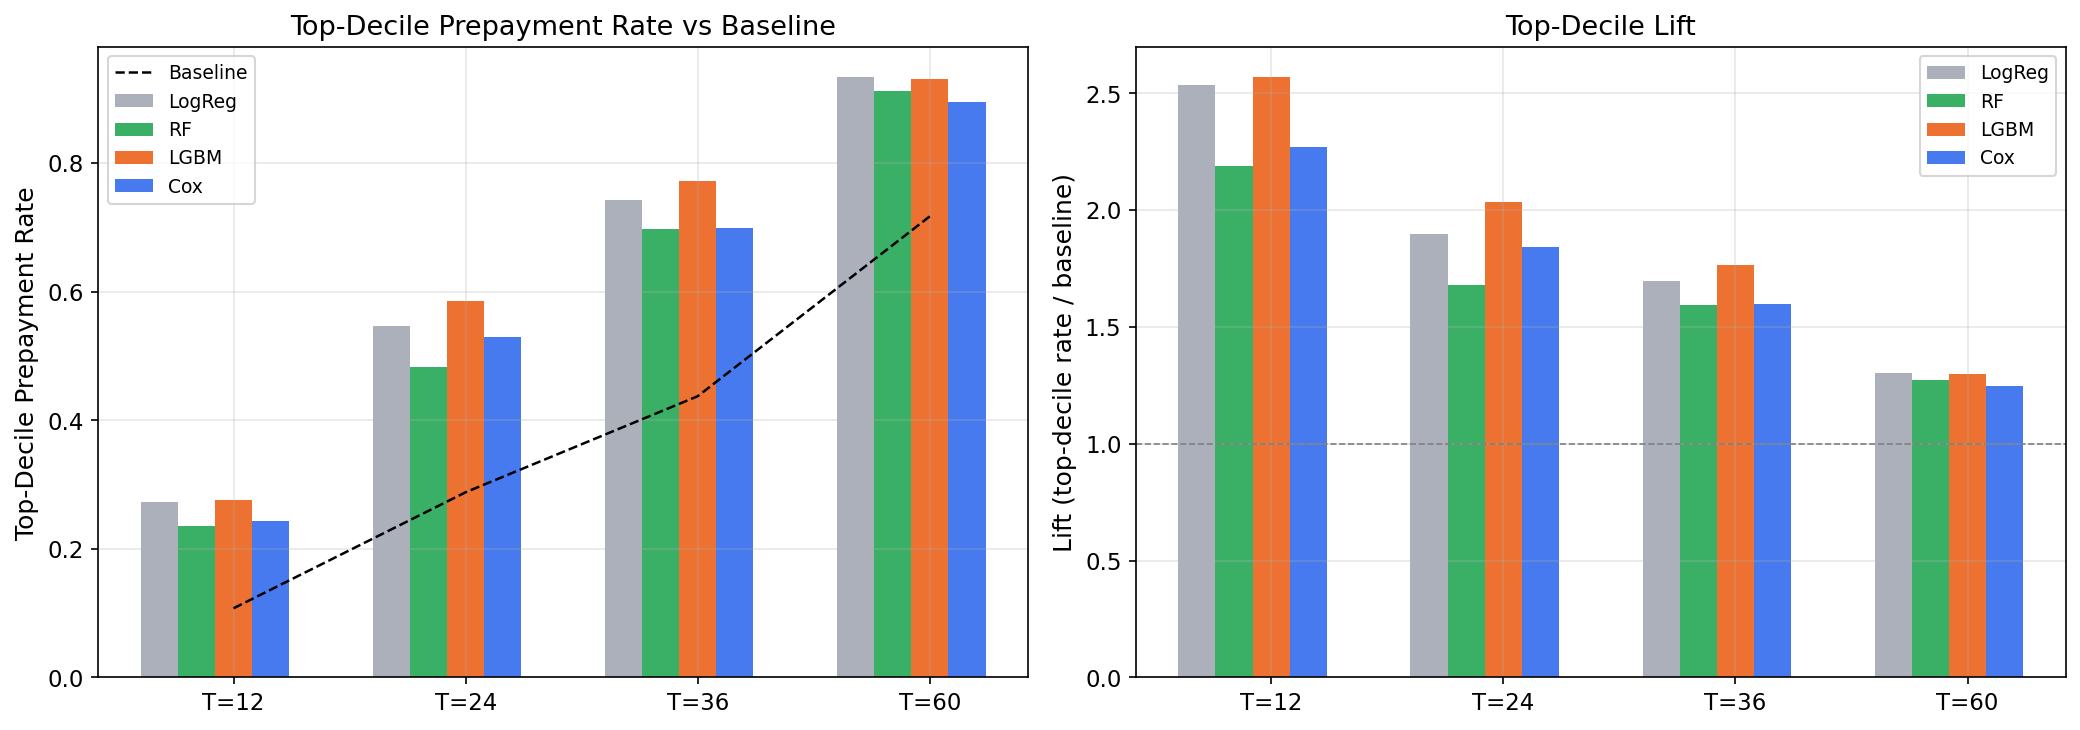
\includegraphics[width=0.65\textwidth]{plots/C_top_decile_lift.png}
\caption{\textbf{Part C: top-decile lift.} Practical-investor metric --- among the top 10\% of test loans ranked by predicted prepay probability, what fraction actually prepays within horizon $T$, divided by the population base rate. Saturation at $T{=}60$ reflects the high base rate (71.7\%).}
\end{figure}

% =================================================================
\section{Part D --- Deep Cox Model}
% =================================================================

\textbf{Architecture.} 3 hidden layers $\times$ 64 ReLU units, batch normalization, dropout 0.1, no output bias (standard DeepSurv setup). 13{,}184 parameters versus 68 for the linear baseline.

\textbf{Training.} pycox's \texttt{CoxPH} with Adam ($\eta = 10^{-3}$), batch 512, max 50 epochs, early-stopping patience 8 on validation partial-likelihood loss. The Cox partial likelihood is computed per minibatch (risk sets are batch-local --- the standard pycox / DeepSurv stochastic approximation). Total CPU runtime: 17 minutes for Deep, 1 minute for Linear baseline. Breslow baseline hazards estimated post-fit on the full training set.

\textbf{D(v) ablation --- Linear vs Deep.} The linear baseline uses the identical pycox infrastructure with \texttt{num\_nodes=[]}, so it is functionally a SGD-fit classical Cox. This is the cleanest possible isolation of the nonlinearity contribution: same data, same optimizer, same baseline-hazard estimator.

\begin{center}
\small
\begin{tabular}{lcccc}
\toprule
Horizon & Linear AUC & Deep AUC & $\Delta$AUC & $\Delta$LogLoss \\
\midrule
12 & 0.6807 & 0.6837 & $+0.0030$ & $-0.0050$ \\
24 & 0.6738 & 0.7007 & $+0.0269$ & $-0.0267$ \\
36 & 0.6772 & 0.7211 & $+0.0439$ & $-0.0517$ \\
60 & 0.6848 & 0.7292 & $+0.0445$ & $-0.1020$ \\
\bottomrule
\end{tabular}
\end{center}

The gap widens monotonically with horizon. The interpretation is clean: at $T{=}12$, the prepayment decision is largely driven by linear effects (rate differential, FICO, balance); but as horizon extends, \emph{interaction} effects between borrower characteristics and the macro/temporal environment become increasingly important, and these are exactly what the network captures.

\textbf{D(iv) head-to-head.} Combined comparison with all Part C models:

\begin{center}
\small
\begin{tabular}{lcccc}
\toprule
Model & T=12 & T=24 & T=36 & T=60 \\
\midrule
Cox & 0.6635 & 0.6571 & 0.6596 & 0.6650 \\
Random Forest & 0.6706 & 0.6519 & 0.6718 & 0.6803 \\
LightGBM & 0.6805 & 0.6738 & 0.6899 & 0.6825 \\
LinearCox (D, ablation) & 0.6807 & 0.6738 & 0.6772 & 0.6848 \\
LogReg & 0.6908 & 0.6670 & 0.6837 & 0.7043 \\
\textbf{DeepCox} & \textbf{0.6837} & \textbf{0.7007} & \textbf{0.7211} & \textbf{0.7292} \\
\bottomrule
\end{tabular}
\end{center}

DeepCox is best at every horizon $\geq 24$ months, often by 0.04--0.05 AUC --- a substantial margin in this domain. At $T{=}12$ LogReg edges it slightly. We also note that LinearCox $>$ Cox at every horizon (by $\sim$0.015--0.020); this is consistent --- both are linear-predictor + Breslow baseline, but LinearCox uses Part C's full encoded feature matrix while the lifelines-fit Cox uses the more parsimonious Part B specification.

\begin{figure}[h]
\centering
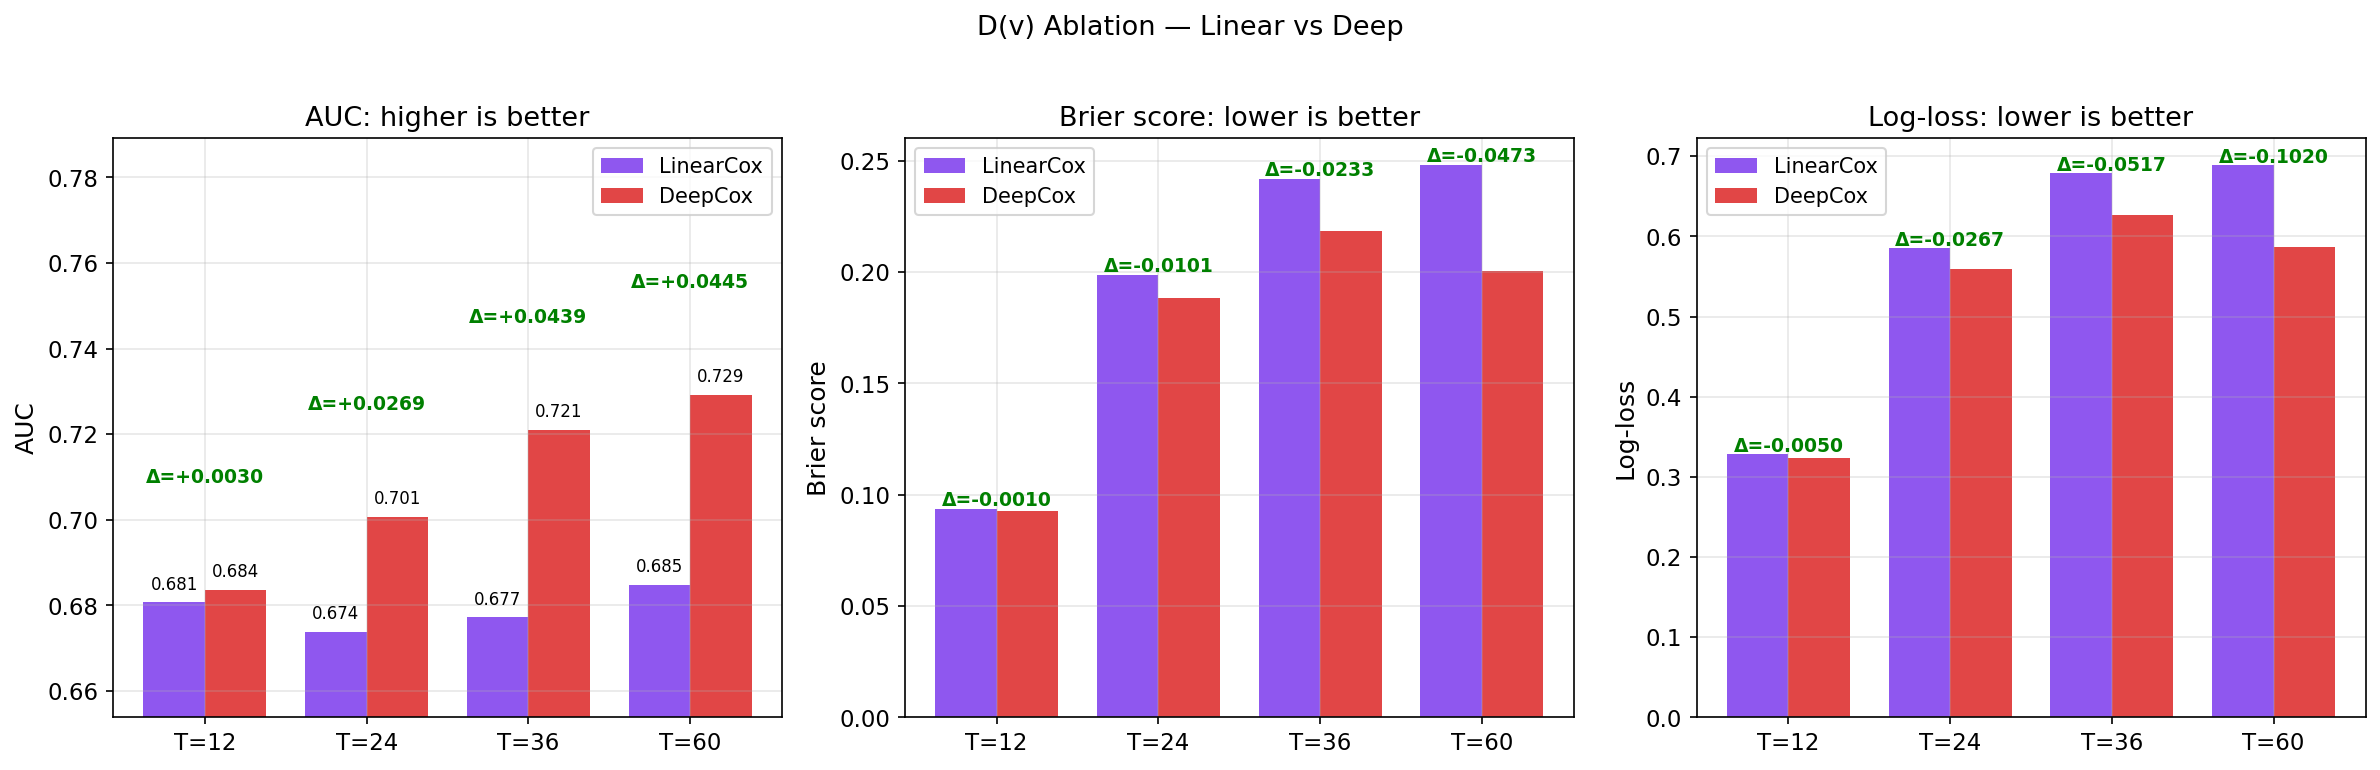
\includegraphics[width=0.48\textwidth]{plots/D_ablation_bars.png}\hfill
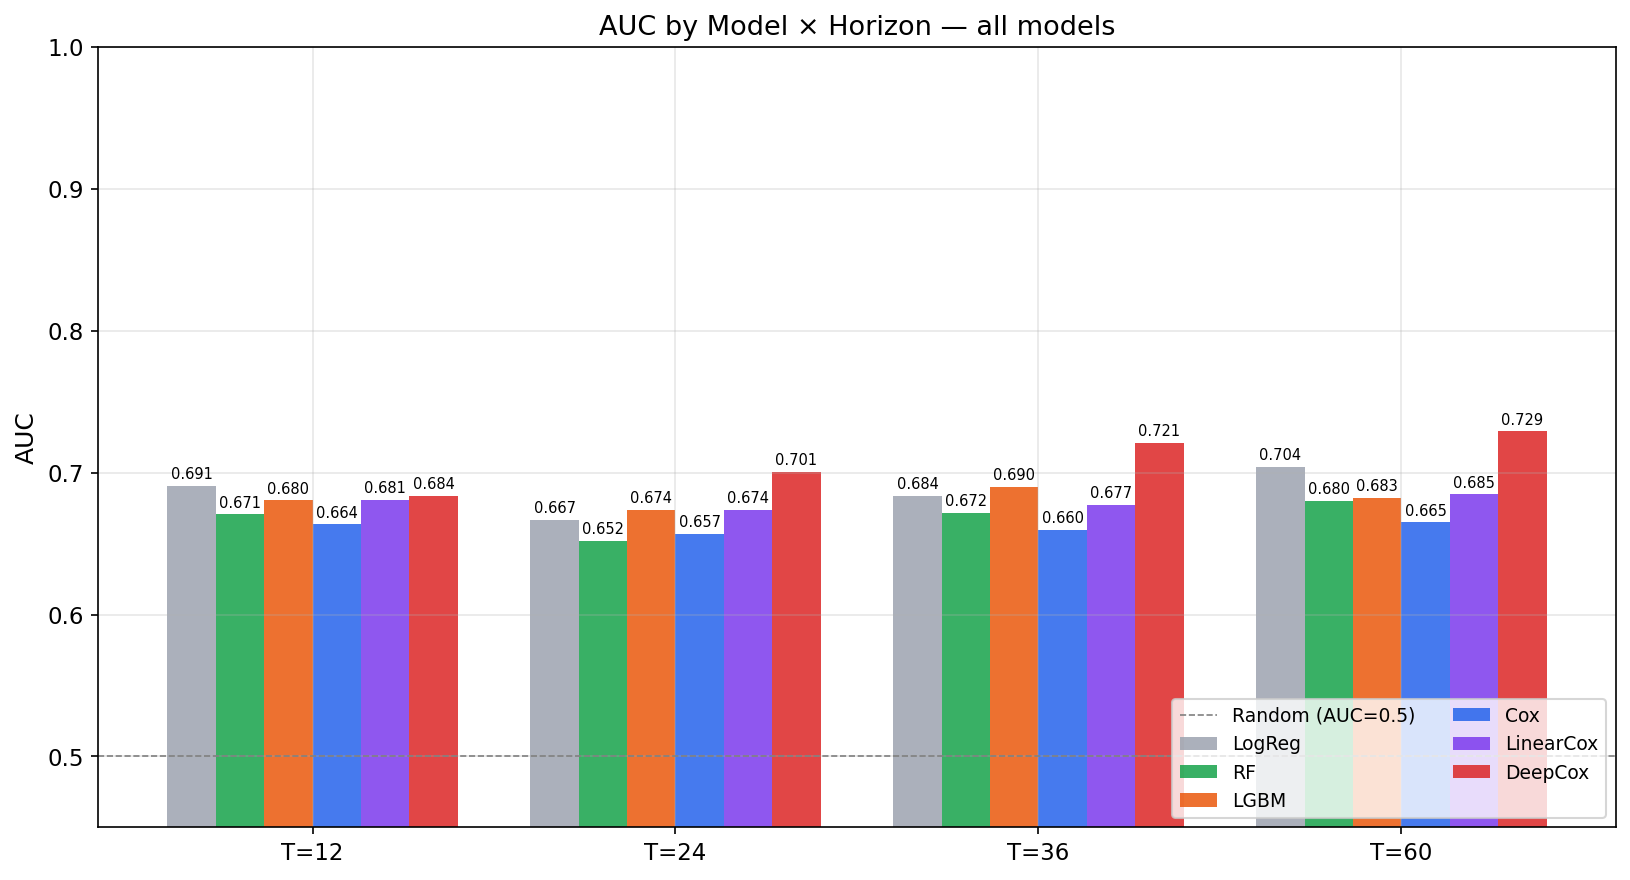
\includegraphics[width=0.48\textwidth]{plots/D_auc_by_horizon.png}
\caption{\textbf{Part D.} Left: D(v) Linear-vs-Deep ablation; Deep gain widens with horizon. Right: head-to-head AUC comparing all six models, with DeepCox winning at long horizons.}
\end{figure}

\textbf{Calibration and top-decile lift.} DeepCox is also the best-calibrated model at long horizons (predicted probabilities track the empirical prepayment rate close to the diagonal in the decile reliability plot). At moderate horizons ($T{=}24$, $T{=}36$) DeepCox also delivers the best top-decile lift among all six models: 2.08$\times$ at $T{=}24$ versus LightGBM's 2.03$\times$ and LogReg's 1.90$\times$. The combination of best AUC, best calibration, and best top-decile lift across long horizons makes DeepCox the dominant model in this study.

\begin{figure}[h]
\centering
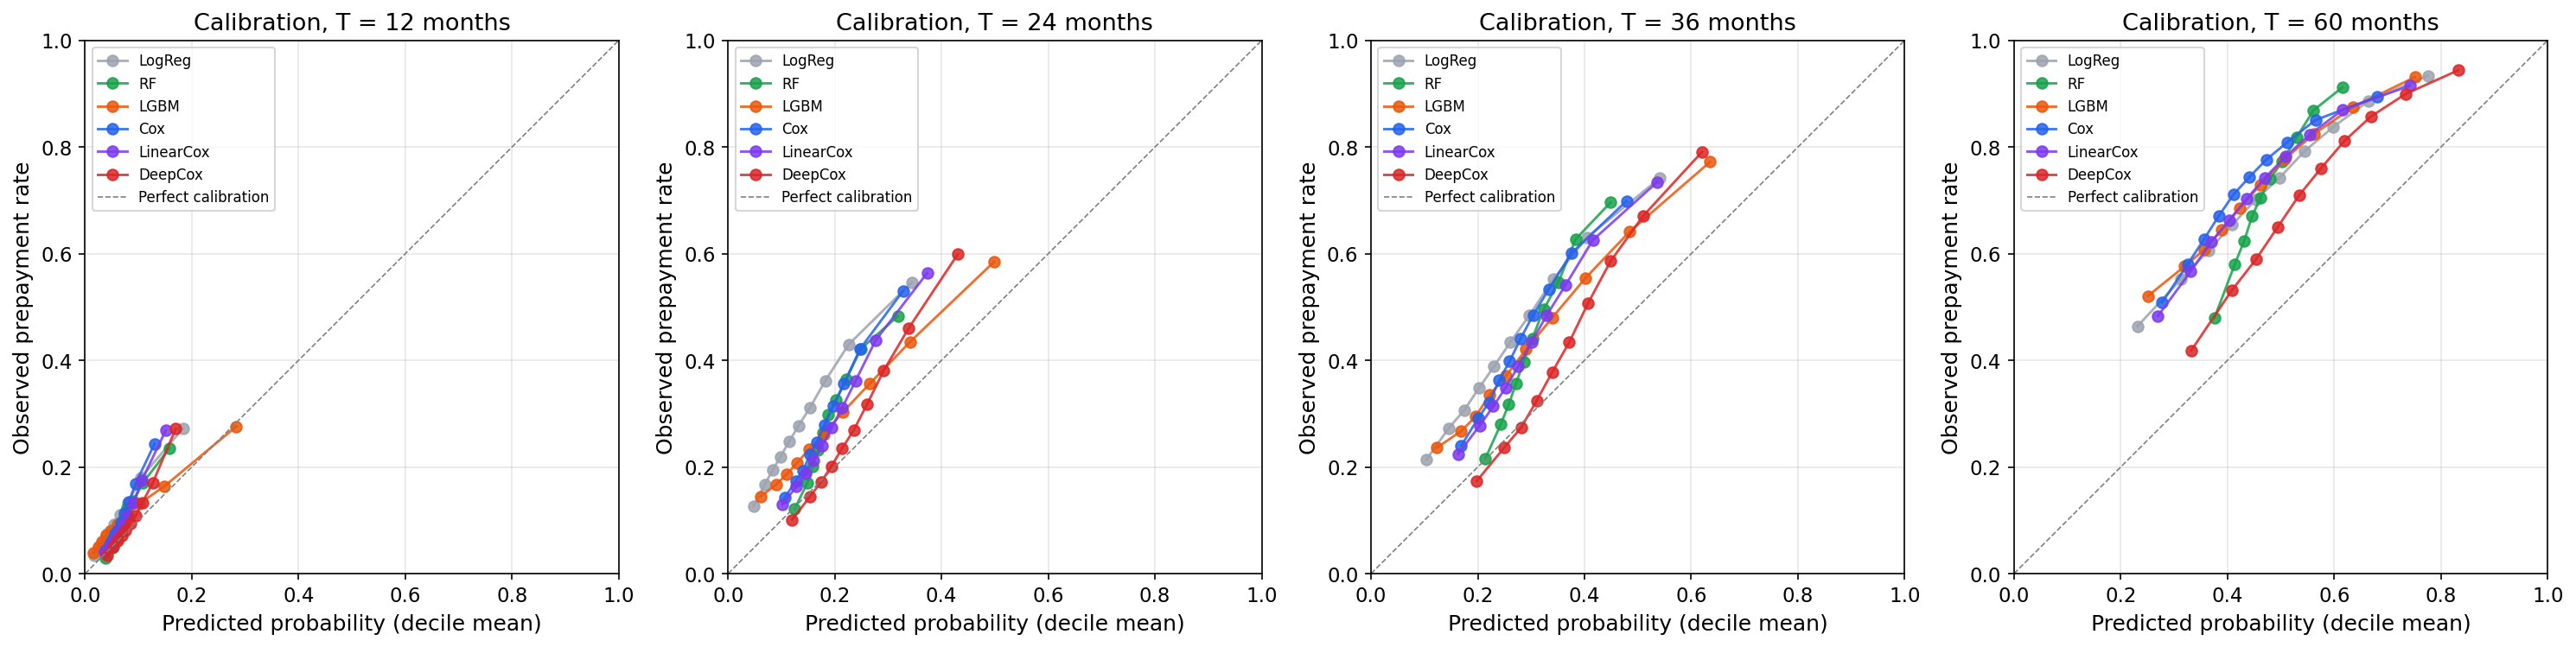
\includegraphics[width=0.49\textwidth]{plots/D_calibration.png}\hfill
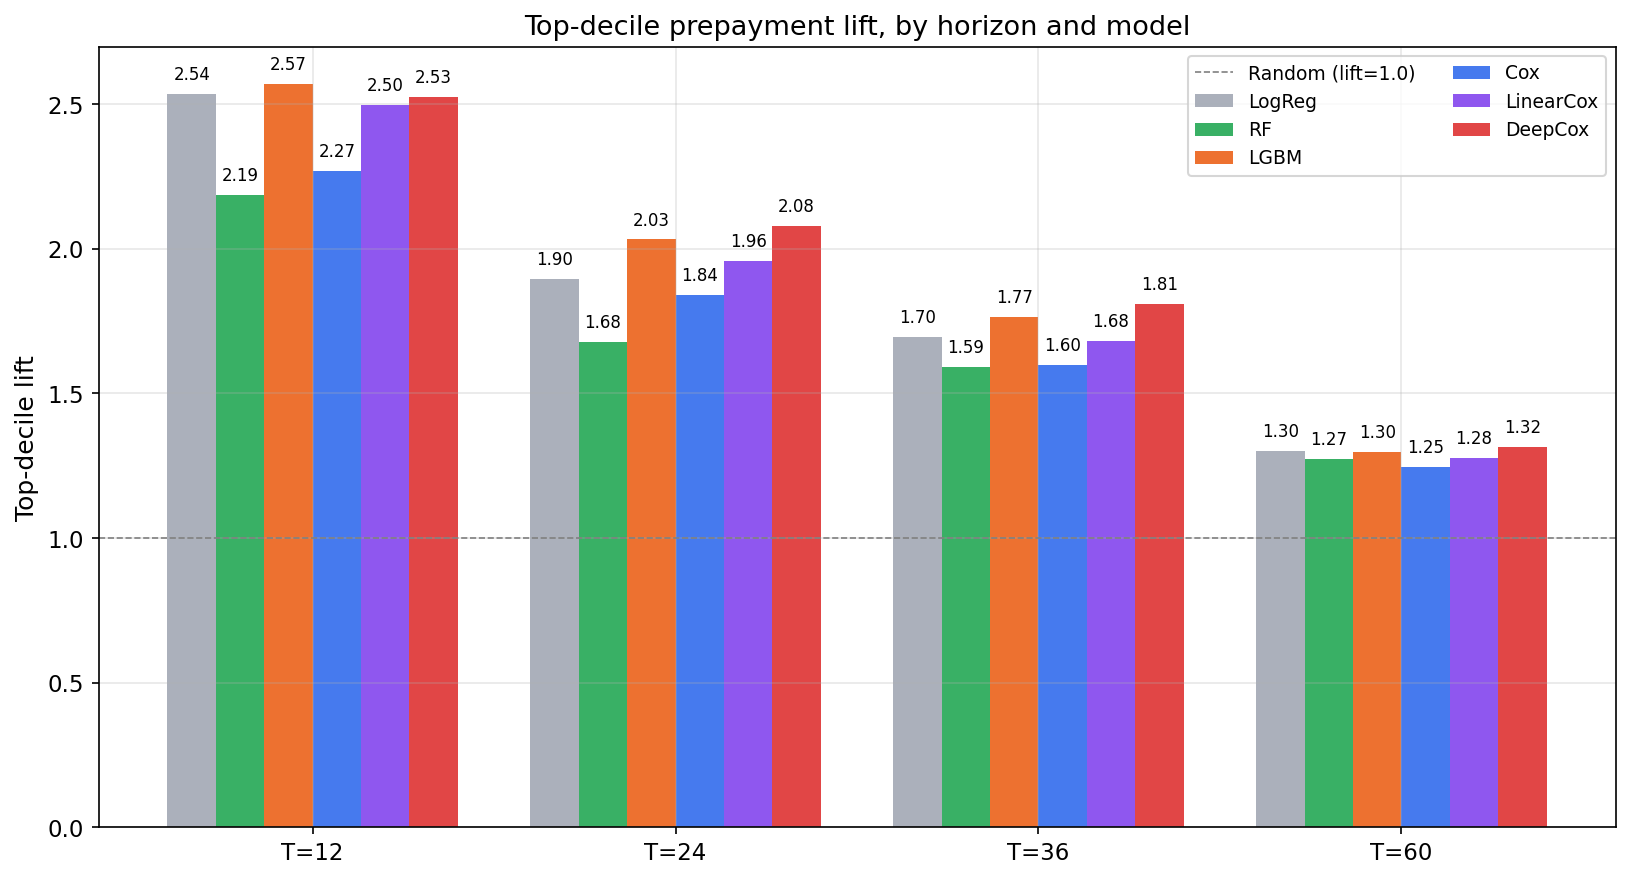
\includegraphics[width=0.49\textwidth]{plots/D_top_decile_lift.png}
\caption{\textbf{Part D supporting plots.} Left: decile calibration for DeepCox vs LinearCox at all horizons. Right: top-decile lift comparison across all six models.}
\end{figure}

% =================================================================
\section{Discussion}
% =================================================================

\textbf{Why Deep wins at long horizons.} A linear Cox model assumes the log-hazard is additive in covariate effects: a loan with a high rate plus high FICO plus low LTV experiences a hazard that is the product of independently-acting multipliers. The data say otherwise: the prepayment incentive of a high origination rate \emph{conditional} on that loan still being alive at $T{=}36$ depends jointly on the borrower's FICO, current balance, and the rate environment they would face in refinancing. The linear model collapses these interactions; the deep model captures them. As horizon extends, more of these compound paths become relevant, so the ablation gap widens.

\textbf{Why short horizons don't show a gap.} At $T{=}12$, the only loans that have prepaid are those with very strong, singular incentive --- typically the highest-rate borrowers facing a meaningfully lower rate environment. These are the easy cases for any model. Tree models find them via single splits; logistic regression finds them via marginal coefficients; the deep network has no extra information to exploit.

\textbf{Comparison with Sadhwani et al.\ (2021).} The Sadhwani--Giesecke--Sirignano paper makes essentially the same finding on a much larger and richer dataset (CoreLogic, 120M+ loans, 272 covariates including zip-code-level macro). Their five-layer network's out-of-sample test-loss reduction over a logistic regression is most pronounced for prepayment among all events --- consistent with our finding that prepayment is where nonlinearities are strongest. Our 0.04--0.05 ΔAUC at long horizons, on a much smaller dataset and with only 68 covariates, is a quantitatively similar gap. The mechanism they identify --- interactions between unemployment and FICO, between LTV and house price appreciation --- aligns with our intuition that interactions become more relevant as horizon extends.

\textbf{Why tree models don't close the gap.} Random Forest and LightGBM are powerful nonlinear learners, but their nonlinearity is axis-aligned: at each node, they split on a single feature. Smooth, multivariate interactions (the kind a sigmoidal or ReLU network with multiple layers naturally represents) require many tree splits to approximate. Sadhwani et al.\ also report that gradient boosting underperforms deep networks for this task. Our finding is consistent: LightGBM tops out at 0.69 AUC; DeepCox reaches 0.73.

\textbf{Why Logistic Regression is competitive at the short end.} At $T{=}12$, prepayment is concentrated in a tail of obvious refi candidates: high original rate, high FICO, large balance, recently originated. Marginal effects are sufficient. As horizon extends and the population at risk thins, the borrower-by-environment interactions matter more, and the linear marginal effects start to lose information.

\textbf{Limitations.}
\begin{enumerate}[leftmargin=1.5em,itemsep=2pt,topsep=2pt]
\item Vintage-macro covariates are static at origination; truly time-varying covariates (current rate differential, current LTV updated by HPI) would likely improve every model but require the loan-month panel ($\sim$3.5B rows in Sadhwani et al.).
\item The cause-specific framing treats competing terminations as censored; a competing-risks framework (Fine--Gray subdistribution hazards or multinomial multi-state models) would model default and prepayment jointly, which is the right framework for credit risk transfer transactions.
\item Mini-batch Cox is a stochastic approximation to the exact partial likelihood. With batch size 512 the approximation is the standard one in the literature, but a sensitivity check across batch sizes 256/1024/2048 would strengthen the conclusions.
\item Vintage-based train/test split means our test set sees a different rate environment than train; this is the right choice for honest out-of-sample evaluation but means absolute AUCs reflect distribution shift, not just model capacity.
\end{enumerate}

\textbf{What we would do next.} Implement (i) competing risks (default vs prepay) as a multi-output network; (ii) genuinely time-varying covariates via the loan-month panel and a recurrent or attention-based survival model; (iii) interest-rate scenario analysis, applying the trained Deep Cox to perturbed rate environments to compute prepayment-incentive curves analogous to those in Sadhwani et al.\ Figure 1.

\subsection{Final results overview}

For ease of comparison, we collect all six models' overall test-set metrics in a single table. Best per-column values are highlighted in bold.

\begin{center}
\small
\begin{tabular}{lcccc|cccc}
\toprule
& \multicolumn{4}{c|}{AUC (higher = better)} & \multicolumn{4}{c}{Brier (lower = better)} \\
Model & T=12 & T=24 & T=36 & T=60 & T=12 & T=24 & T=36 & T=60 \\
\midrule
Cox       & 0.6635 & 0.6571 & 0.6596 & 0.6650 & 0.0949 & 0.2048 & 0.2527 & 0.2659 \\
RF        & 0.6706 & 0.6519 & 0.6718 & 0.6803 & 0.0939 & 0.2050 & 0.2475 & 0.2456 \\
LGBM      & 0.6805 & 0.6738 & 0.6899 & 0.6825 & \textbf{0.0916} & 0.1941 & 0.2343 & 0.2503 \\
LinearCox & 0.6807 & 0.6738 & 0.6772 & 0.6848 & 0.0935 & 0.1986 & 0.2419 & 0.2479 \\
LogReg    & \textbf{0.6908} & 0.6670 & 0.6837 & 0.7043 & 0.0932 & 0.2119 & 0.2500 & 0.2366 \\
\textbf{DeepCox} & 0.6837 & \textbf{0.7007} & \textbf{0.7211} & \textbf{0.7292} & 0.0925 & \textbf{0.1885} & \textbf{0.2186} & \textbf{0.2007} \\
\bottomrule
\end{tabular}
\end{center}

\textbf{Reading guide.} Two distinct stories: at short horizons (T=12), LogReg has the best AUC and LightGBM has the best Brier --- both linear-or-near-linear models. At moderate-to-long horizons (T=24, 36, 60), DeepCox wins both AUC and Brier (and log-loss, calibration, top-decile lift --- in the underlying data tables not shown here for space). The transition between these regimes happens between $T{=}12$ and $T{=}24$ months, which is where prepayment shifts from being concentrated in obvious-incentive borrowers to being distributed across the broader population.

% =================================================================
\section{Reproducibility and Engineering Notes}
% =================================================================

\textbf{Pipeline structure.} The full pipeline is six scripts plus four plotting notebooks, running end-to-end in approximately 50 minutes on a single CPU machine. Each compute script writes parquet outputs only and contains no plotting; plotting is delegated to per-part Jupyter notebooks that read from the corresponding \texttt{results\_*/} folder. This compute/plot separation makes both halves easier to iterate on independently.

\textbf{Single source of truth.} A canonical split file (\texttt{canonical\_split.parquet}) records the train/test partition used by Parts C and D. Part D's \texttt{restrict\_to\_canonical\_split} loads this file and reorders rows to match Part C exactly, with a row-by-row alignment assertion that fails loudly if the splits diverge. Encoders fit on training data are persisted as \texttt{encoders.pkl} and loaded by Part D --- so test-set features are encoded with the identical fitted statistics, eliminating one common source of leakage.

\textbf{Engineering challenges.} Three were significant: (i) \textbf{memory} --- the full survival table is 31.7M rows $\times$ 39 columns; we used polars for the build (faster and more memory-efficient than pandas) and float32 for numerical features; (ii) \textbf{validation leakage} --- Part D's val slice is carved from train \emph{before} feature transformation and standardization, with the scaler fit only on the inner train; (iii) \textbf{cross-AI verification} --- the code was reviewed iteratively across two LLM chats. Critical bugs caught: encoder-fit-before-split leakage in original Part C, validation-after-standardization in original Part D, and a sentinel-cleaning ordering bug in Part B (\texttt{has\_MI} flag was being computed before MI=999 sentinels were cleaned).

All hyperparameters and CLI flags are documented in \texttt{D\_model\_meta.json}, including feature names, scaler statistics, training configuration, and runtime measurements.

\begin{thebibliography}{9}
\small
\bibitem{sadhwani2021}
Sadhwani, A., Giesecke, K., \& Sirignano, J. (2021).
\textit{Deep Learning for Mortgage Risk}. Journal of Financial Econometrics 19(2), 313--368.

\bibitem{deepsurv}
Katzman, J. L., Shaham, U., Cloninger, A., Bates, J., Jiang, T., \& Kluger, Y. (2018).
\textit{DeepSurv: personalized treatment recommender system using a Cox proportional hazards deep neural network}. BMC Medical Research Methodology 18(1), 24.

\bibitem{lifelines}
Davidson-Pilon, C. (2019).
\textit{lifelines: survival analysis in Python}. Journal of Open Source Software 4(40), 1317.

\bibitem{pycox}
Kvamme, H., Borgan, {\O}., \& Scheel, I. (2019).
\textit{Time-to-event prediction with neural networks and Cox regression}. Journal of Machine Learning Research 20(129), 1--30.

\bibitem{kalbfleischprentice}
Kalbfleisch, J. D., \& Prentice, R. L. (2002).
\textit{The Statistical Analysis of Failure Time Data}, 2nd ed., Wiley.

\bibitem{chen2024}
Chen, G. (2024).
\textit{An Introduction to Deep Survival Analysis Models for Predicting Time-to-Event Outcomes}.
\end{thebibliography}

\end{document}
